\documentclass[12pt,a4paper]{report}

\usepackage{xcolor}
% ---------------- Packages ----------------
\usepackage{graphicx}
\usepackage{geometry}
\usepackage{setspace}
\usepackage{tocloft}
\usepackage{enumitem}
\usepackage{needspace}
\usepackage{pdfpages}
\usepackage{titlesec}
\usepackage{fancyhdr}
\usepackage{amsmath,amssymb}
\usepackage{listings}
\usepackage{tabularx}
\usepackage{booktabs}
\usepackage{longtable}
\usepackage{url}
\usepackage[hidelinks]{hyperref}
\usepackage{ragged2e}
\usepackage{array}
\usepackage{float}

% ---------------- Page Setup ----------------
\geometry{
    left=1.25in,
    right=1in,
    top=1in,
    bottom=1in
}

\onehalfspacing
\setlength{\parindent}{0pt}
\setlength{\parskip}{8pt}
\setlength{\headheight}{15pt}

% ---------------- Custom Font Command ----------------
\newcommand{\headingSixteen}[1]{{\fontsize{16pt}{18pt}\selectfont\textbf{#1}}}
\newcommand{\headingFourteen}[1]{{\fontsize{14pt}{16pt}\selectfont\textbf{#1}}}

% ---------------- Justified Table Column Types ----------------
\newcolumntype{J}{>{\justifying\arraybackslash}X}
\newcolumntype{L}[1]{>{\raggedright\arraybackslash}p{#1}}
\newcolumntype{C}[1]{>{\raggedright\ttfamily\footnotesize\arraybackslash}p{#1}}

\renewcommand{\arraystretch}{1.3}

\urlstyle{same}
\def\UrlBreaks{\do\/\do\-\do\_\do\.\do\:\do\(\do\)}
\Urlmuskip=0mu plus 1mu

% ---------------- Table of Contents Formatting ----------------
\renewcommand{\contentsname}{TABLE OF CONTENTS}

\setlength{\cftbeforetoctitleskip}{0pt}
\setlength{\cftaftertoctitleskip}{20pt}
\setlength{\cftchapindent}{0pt}
\setlength{\cftsecindent}{1.5em}

\renewcommand{\cftchapfont}{\bfseries}
\renewcommand{\cftchappagefont}{\bfseries}
\renewcommand{\cftdotsep}{1}

\setlength{\cftbeforechapskip}{6pt}

\makeatletter
\renewcommand{\@cftmaketoctitle}{%
  \begin{center}
    \fontsize{16pt}{18pt}\selectfont\textbf{\contentsname}
  \end{center}
  \vspace{10pt}
}
\makeatother

% ==========================================================
% CHAPTER TITLE PAGE FORMATTING
% ==========================================================

\titleformat{\chapter}[display]
    {\bfseries\centering\fontsize{16pt}{18pt}\selectfont}
    {\chaptertitlename\ \thechapter}
    {10pt}
    {\fontsize{16pt}{18pt}\selectfont}

\titleformat{\section}
    {\bfseries\fontsize{14pt}{16pt}\selectfont}
    {\thesection}
    {1em}
    {}

\titleformat{\subsection}
    {\bfseries\fontsize{12pt}{14pt}\selectfont}
    {\thesubsection}
    {1em}
    {}

\newcommand{\chaptertitlepage}[1]{%
    \cleardoublepage
    \thispagestyle{empty}
    \null
    \vfill
    \begin{center}
        {\fontsize{16pt}{18pt}\selectfont\bfseries
        CHAPTER \thechapter}\\[0.5cm]
        {\fontsize{16pt}{18pt}\selectfont\bfseries
        #1}
    \end{center}
    \vfill
    \null
    \clearpage
}

% ---------------- Header & Footer ----------------

\fancypagestyle{maincontent}{
\fancyhf{}
\fancyhead[R]{\small Smart Motion Detection Alarm System using IoT}

\fancyfoot[L]{\small \textit{Saintgits College of Engineering (Autonomous)}}
\fancyfoot[R]{\small \thepage}
\renewcommand{\headrulewidth}{0.0pt}
\renewcommand{\footrulewidth}{0.0pt}
}


% ---------------- Bibliography Spacing ----------------
\makeatletter
\renewenvironment{thebibliography}[1]
  {\section*{}\@mkboth{}{}%
   \list{\@biblabel{\@arabic\c@enumiv}}%
        {\settowidth\labelwidth{\@biblabel{#1}}%
         \leftmargin\labelwidth
         \advance\leftmargin\labelsep
         \itemsep=0.6\baselineskip
         \usecounter{enumiv}%
         \let\p@enumiv\@empty
         \renewcommand\theenumiv{\@arabic\c@enumiv}}%
   \sloppy}
  {\endlist}
\makeatother

% ---------------- Code Snippet Formatting ----------------
\definecolor{codegray}{rgb}{0.5,0.5,0.5}
\definecolor{codepurple}{rgb}{0.58,0,0.82}
\definecolor{backcolour}{rgb}{0.96,0.97,0.98}

\lstdefinestyle{codeStyle}{
    backgroundcolor=\color{backcolour},
    commentstyle=\color{codegray},
    keywordstyle=\color{magenta},
    numberstyle=\tiny\color{codegray},
    stringstyle=\color{codepurple},
    basicstyle=\ttfamily\footnotesize,
    breakatwhitespace=false,
    breaklines=true,
    keepspaces=true,
    numbers=left,
    numbersep=5pt,
    showspaces=false,
    showstringspaces=false,
    showtabs=false,
    tabsize=2
}

\lstset{style=codeStyle}

\hyphenpenalty=200
\exhyphenpenalty=200
\tolerance=1200
\emergencystretch=2em

% ==========================================================
% DOCUMENT
% ==========================================================

\begin{document}

\justifying

% ==========================================================
% PAGE 1 : TITLE PAGE
% ==========================================================

\thispagestyle{empty}

\begin{center}

\vspace*{-0.8cm}

{\fontsize{14pt}{16pt}\selectfont
\textbf{PERSONALIZED LEARNING TRACKS (TRACK 3)}}\\[0.2cm]

{\fontsize{14pt}{16pt}\selectfont
\textbf{SDG PROJECT REPORT}}\\[0.15cm]

{\fontsize{12pt}{14pt}\selectfont
\textbf{ON}}\\[0.15cm]

{\fontsize{14pt}{16pt}\selectfont
\textbf{\textcolor{blue}{ SMART MOTION DETECTION ALARM SYSTEM USING IOT}}}\\[0.45cm]

{\fontsize{12pt}{14pt}\selectfont
\textbf{Submitted By}}\\[0.1cm]

{\fontsize{13pt}{15pt}\selectfont
\textbf{\textcolor{blue}{ARJUN GHOSH - MGP25MCA-2023}}}\\[0.45cm]

{\fontsize{12pt}{14pt}\selectfont
\textbf{To}}\\[0.1cm]

\textit{the APJ Abdul Kalam Technological University in partial}\\
\textit{fulfillment of the requirements for the award of the degree of}\\[0.25cm]

{\fontsize{13pt}{15pt}\selectfont
\textbf{MASTER OF COMPUTER APPLICATIONS}}\\[0.45cm]

{\fontsize{12pt}{14pt}\selectfont
\textbf{Under the guidance of}}\\[0.1cm]

{\fontsize{13pt}{15pt}\selectfont
\textbf{\textcolor{blue}{Dr. JACOB ZACHARIA}}}\\

{\fontsize{12pt}{14pt}\selectfont
\textcolor{blue}{Assistant Professor}}\\[0.9cm]

\includegraphics[width=3.2cm]{Saintgits logo New.png}\\[0.50cm]

{\fontsize{12pt}{14pt}\selectfont
\textbf{DEPARTMENT OF COMPUTER APPLICATIONS}}\\[0.1cm]

{\fontsize{13pt}{15pt}\selectfont
\textbf{SAINTGITS COLLEGE OF ENGINEERING (AUTONOMOUS)}}\\

{\fontsize{11pt}{13pt}\selectfont
\textbf{Pathamuttom, Kottayam, Kerala -- 686532}}\\[0.2cm]

{\fontsize{10pt}{12pt}\selectfont
\textit{(Approved by AICTE and affiliated to APJ Abdul Kalam Technological University)}}\\[0.5cm]

{\fontsize{14pt}{16pt}\selectfont
\textbf{SEPTEMBER 2026}}

\end{center}

% ==========================================================
% PAGE 2 : BONAFIDE
% ==========================================================

\newpage
\thispagestyle{empty}

\begin{center}
\fontsize{16pt}{18pt}\selectfont
\textbf{SAINTGITS COLLEGE OF ENGINEERING (AUTONOMOUS)}\\
Kottukulam Hills, Pathamuttom, Kottayam, Kerala -- 686532
\end{center}

\vspace{0.2cm}

\begin{center}
\includegraphics[width=4.2cm]{Saintgits logo New.png}
\end{center}

\vspace{0.1cm}

\begin{center}
\fontsize{16pt}{18pt}\selectfont
\textbf{BONAFIDE CERTIFICATE}
\end{center}

\vspace{0.4cm}

{\sloppy\justifying

Certified that the report entitled
\textbf{``Smart Motion Detection Alarm System using IoT''}
submitted by
\textbf{Arjun Ghosh (Reg~No:\ MGP25MCA-2023)}
to the APJ Abdul Kalam Technological University in partial fulfillment of the
requirements for the award of the Degree of
\textbf{Master of Computer Applications}
is a bonafide record of the
\textbf{Social Immersion Sustainable Development Goals (SDG)}
project work carried out by him under our guidance and supervision.
This report in any form has not been submitted to any other University or Institute
for any purpose.\par}

\vspace{2.2cm}

\noindent
\begin{minipage}[t]{0.45\textwidth}
\raggedright
\textbf{Dr. Jacob Zacharia}\\
Internal Guide
\end{minipage}
\hfill
\begin{minipage}[t]{0.45\textwidth}
\raggedleft
\textbf{Ms. Ankitha Philip}\\
SDG Project Coordinator
\end{minipage}

\vspace{2.2cm}

\noindent
\begin{center}
\begin{minipage}{0.55\textwidth}
\centering
\textbf{Dr. Rani Saritha R}\\
Head of the Department\\
\end{minipage}
\end{center}

\vspace{1.5cm}

% ==========================================================
% PAGE 3 : ACKNOWLEDGEMENT
% ==========================================================

\newpage
\thispagestyle{empty}

\begin{center}
\fontsize{16pt}{18pt}\selectfont
\textbf{ACKNOWLEDGEMENT}
\end{center}

\vspace{1cm}

First of all, I thank the Lord Almighty for His grace, strength and hope, which helped me complete this work. I am sincerely grateful to \textbf{Dr. Sudha T}, Principal, Saintgits College of Engineering (Autonomous), for her support during this project, and also to the management for providing the required facilities.

I am also thankful to \textbf{Prof. Mini Punnoose}, Director MCA, Department of Computer Applications, Saintgits College of Engineering (Autonomous), for her constant encouragement. I thank \textbf{Dr. Rani Saritha R}, Head of the Department, Department of Computer Applications, Saintgits College of Engineering (Autonomous), for her support and guidance.

I am very grateful to \textbf{Dr. Jacob Zacharia}, my SDG Project Guide, and \textbf{Ms. Ankitha Philip}, the SDG Project Coordinator, for their guidance, help, suggestions and regular review of my work.

I also thank everyone else who helped me, especially my parents and friends. Their support, suggestions and encouragement made it possible to finish this project report.

\vspace{2cm}

\begin{flushright}
\textbf{Arjun Ghosh}\\
(MGP25MCA2023)
\end{flushright}

% ==========================================================
% PAGE 4 : ABSTRACT
% ==========================================================

\newpage
\thispagestyle{empty}

\begin{center}
\fontsize{16pt}{18pt}\selectfont
\textbf{ABSTRACT}
\end{center}

\vspace{1cm}

\textbf{Smart Motion Detection Alarm System using IoT} is a Windows desktop application for home security. It uses ESP32-based PIR motion sensors, an optional webcam, and a floor-plan screen where the user can see activity. Many homes and small buildings now use low-cost IoT devices for safety. What they often lack is one place that can take sensor events, show them on a floor plan, keep a history, and send alerts when the system is armed.

In this system, the user logs in, places PIR sensors and cameras on an isometric floor plan, and receives live motion events from the ESP32 firmware through a serial connection. Optional camera snapshots can also be saved. Each event is given a risk level using Home/Away mode and time-of-day rules. The user can later check history, analytics and PDF reports. When the console is armed (Away mode), motion alerts can be sent to Telegram, Discord and Twilio WhatsApp, based on the set schedule and cooldown time.

The application is written in Python~3. CustomTkinter is used for the desktop interface, MySQL for storing data, pyserial for talking to the ESP32, OpenCV for camera capture, and fpdf2 for PDF reports. Telegram and Discord alerts go through HTTP APIs, and WhatsApp alerts use the Twilio API. Risk scoring is done by a separate RiskEngine using simple rules. AI person detection is not part of this version and is left for later work.

\vspace{0.5cm}

This project is linked to \textbf{SDG 11 -- Sustainable Cities and Communities}, because it helps people notice unexpected motion sooner and keep a clear record of events. It also supports \textbf{SDG 9 -- Industry, Innovation and Infrastructure} by showing how low-cost sensors, a desktop program and mobile alerts can work together. The aim is a simple, paperless way to watch home security from one console.

% ==========================================================
% TABLE OF CONTENTS
% ==========================================================

\clearpage
\pagenumbering{gobble}
\pagestyle{empty}

\tableofcontents

\clearpage

\listoffigures
\listoftables

\clearpage

\pagenumbering{arabic}
\pagestyle{maincontent}

% ==========================================================
% CHAPTER 1
% ==========================================================

\refstepcounter{chapter}
\addcontentsline{toc}{chapter}{CHAPTER \thechapter: INTRODUCTION}

\cleardoublepage
\thispagestyle{empty}

\null
\vfill

\begin{center}
    {\fontsize{16pt}{18pt}\selectfont\bfseries
    CHAPTER 1}\\[0.5cm]

    {\fontsize{16pt}{18pt}\selectfont\bfseries
    INTRODUCTION}
\end{center}

\vfill
\null

\clearpage

\section{Project Overview}

Home and building security now depends a lot on motion sensors, cameras and phone alerts. Cheap PIR (Passive Infrared) modules and ESP32 boards can detect movement, but they are hard to use on their own. Without one main screen, it is difficult to see \emph{where} the motion happened, to keep a proper history, or to decide when a phone alert should be sent. Simple sensor kits usually do not show a floor plan, do not tell if the house is Home or Away, do not make reports, and do not control alerts on more than one channel.

Smart Motion Detection Alarm System using IoT is built to fill this gap. It is a Windows desktop console. It connects to ESP32 PIR firmware over USB serial, can take webcam snapshots if a camera is present, and lets the user place devices on an isometric floor plan. Every motion event is stored in MySQL. Live alerts, history, analytics and PDF reports are shown in the same application. The admin can arm (Away) or disarm (Home) mobile alerts, set Telegram, Discord and WhatsApp channels, and use a schedule and cooldown so that messages are useful and not too frequent.

A rule-based RiskEngine gives each event a Low, Medium, High or Critical level. It looks at whether the system is armed, the time of day, and whether the sensor is already placed on the floor plan. When motion is detected, a short five-step animation runs on the floor plan, and an Active Alert card appears. On the Command Center, camera and serial health widgets show if the hardware and database are working.

The software is built with Python~3 and CustomTkinter. MySQL stores the data. pyserial reads the ESP32 messages. OpenCV and Pillow handle images. bcrypt hashes passwords, and fpdf2 makes PDF reports. The ESP32 firmware is written in Arduino C++ and sends \texttt{MOTION,\{location\},\{sensorID\}} at 115200 baud. Mobile alerts are sent from a background queue, so the screen does not freeze.

\section{Objectives}

The main aim of this project is to build one desktop console that makes IoT motion monitoring easy to understand and easy to act on. It should keep a reliable log, show risk in a simple way, and send mobile alerts when needed.

The specific objectives of the system are:

\begin{enumerate}
\item To provide a secure login screen. Camera and serial services should start after login and stop after logout.

\item To connect ESP32 PIR firmware through a COM port and baud rate that can be changed in Settings, and to read live \texttt{MOTION} messages into the application.

\item To show an isometric floor plan with zoom, pan, fullscreen and Place Mode, so PIR sensors and cameras can be positioned on it.

\item To keep floor-plan markers in sync with the Sensors and Cameras pages, so the device list stays consistent.

\item To animate motion at the matching marker, show an Active Alert card, and store the event in MySQL, with an optional camera snapshot.

\item To assign a risk level (Low / Medium / High / Critical) using Home/Away mode, night-time rules, and a check of whether the sensor is known.

\item To send mobile alerts on Telegram, Discord and Twilio WhatsApp only when the system is Armed (Away), and to respect the schedule window and cooldown.

\item To provide Security Events history, Analytics with daily and hourly charts, and Reports that can be exported as PDF for a selected date range.

\item To provide Settings for serial reconnect, camera index, floor-plan image change, admin password change, and alert credentials.

\item To keep an AI Security page as a placeholder for later person-detection work, without claiming that AI detection is already working in version 1.
\end{enumerate}

\section{Scope of the Project}

This project covers a Windows desktop console for IoT motion detection and home security. It includes ESP32 serial connection, floor-plan display, MySQL event history, rule-based risk scoring, and optional mobile alerts. Version 1 is a working prototype. It shows how sensor input, live monitoring, logging, analytics and alert rules can sit in one application.

For the operator, the scope includes login, Command Center health widgets, live monitoring, floor-plan placement and animation, sensors and cameras list, history and event details, analytics charts, PDF reports, and settings for hardware and mobile channels.

On the hardware side, the ESP32 PIR firmware reports location and sensor ID over serial. An optional local webcam can take snapshots when motion is detected. The data stored in MySQL includes users, devices, floor plans, rooms, the motion log, and system settings.

The present version focuses on reliable motion capture, a clear floor-plan view, risk labels, and controlled mobile alerts. It does not include cloud accounts for many users, automatic police dispatch, network-level intrusion prevention, or AI person detection. Those items are noted as future work.

% ==========================================================
% CHAPTER 2
% ==========================================================

\refstepcounter{chapter}
\addcontentsline{toc}{chapter}{CHAPTER \thechapter: SUSTAINABLE DEVELOPMENT GOAL}

\cleardoublepage
\thispagestyle{empty}

\null
\vfill

\begin{center}
    {\fontsize{16pt}{18pt}\selectfont\bfseries
    CHAPTER 2}\\[0.5cm]

    {\fontsize{16pt}{18pt}\selectfont\bfseries
    SUSTAINABLE DEVELOPMENT GOAL}
\end{center}

\vfill
\null

\clearpage

\section{Overview of Sustainable Development Goal}

The United Nations Sustainable Development Goals (SDGs) are a common plan for peace and better living for people and the planet. A technology project can help when it makes homes safer, gives people clearer information, or uses simple digital tools in a useful way. Smart Motion Detection Alarm System using IoT is treated as an SDG project because safer homes and a practical IoT monitoring setup support community well-being and also show a working digital system.

This chapter names the selected SDGs, the problems the project tries to solve, how the system helps those goals, and the likely social and environmental effect of keeping motion records and alerts in digital form.

\section{Selected SDG(s)}

Smart Motion Detection Alarm System using IoT is linked to two Sustainable Development Goals:

\subsection{SDG 11 -- Sustainable Cities and Communities}
SDG 11 is about making cities and settlements inclusive, safe, resilient and sustainable. Safety in homes and small buildings is a real part of that. Smart Motion Detection Alarm System using IoT helps by giving people earlier notice of unexpected motion, a clear view of where it happened, and a saved history so they can respond with information rather than panic.

\subsection{SDG 9 -- Industry, Innovation and Infrastructure}
SDG 9 is about strong infrastructure, industry that more people can take part in, and innovation. Low-cost ESP32 and PIR hardware, open desktop software, and common notification APIs show that an IoT setup can be built without being locked to one vendor. Smart Motion Detection Alarm System using IoT supports SDG 9 by joining sensors, serial communication, a database, a floor-plan view and mobile channels in one academic prototype that others can also follow.

\section{Problem Addressed}

This section lists the home IoT security problems that Smart Motion Detection Alarm System using IoT tries to solve.

\subsection{Fragmented Sensor and Camera Tools}
Many houses use different apps for sensors, cameras and chat bots. Smart Motion Detection Alarm System using IoT puts serial PIR events, optional webcam capture, floor-plan placement, history and alerts in one console.

\subsection{Lack of Spatial Context for Motion}
A beep or a serial line does not show \emph{which room} was triggered. The isometric floor plan with device markers and animation maps each sensor ID to a place on the map, so the room is visible.

\subsection{Noisy or Uncontrolled Notifications}
If mobile alerts are always on, people get tired of them. If they are never on, Away-mode incidents are missed. Armed/Disarmed mode, optional night schedules, and cooldown rules send outside alerts only when the policy allows it.

\subsection{Limited Historical Visibility}
Without a database timeline, the user cannot look back at when and where motion happened. MySQL motion logging, unread badges, event-detail windows, analytics charts and PDF reports fill this gap.

\subsection{Unclear Risk Context}
Not every motion event is equally serious. The RiskEngine raises the risk when the system is Armed, raises it further at night, and raises it again if an unknown sensor appears.

\subsection{Weak Hardware Health Awareness}
A disconnected COM port or camera can stay unnoticed until an incident is missed. Command Center health widgets for ESP32, camera and database status help the operator see if the system is ready.

\section{Contribution of the Proposed Project towards the SDG(s)}

Smart Motion Detection Alarm System using IoT helps SDG 11 by supporting safer homes and small buildings. It helps SDG 9 by showing an IoT setup built from hardware and software that students and small users can actually obtain.

\subsection{Strengthening Household and Premises Safety (SDG 11)}
The console follows a simple path: motion is detected, shown on the floor plan, given a risk label, saved, optionally snapshotted, and---when Armed---sent to the chosen mobile channels. History and reports give occupants and caretakers a record of activity, which supports safer living.

\subsection{Demonstrating Innovative IoT Infrastructure (SDG 9)}
ESP32 firmware, serial messages, MySQL storage, a desktop floor plan and multi-channel alerts show how a monitoring setup can be put together and later extended. Separate notifiers and a separate RiskEngine leave room for more sensors and for AI modules later.

\section{Expected Social and Environmental Impact}

Smart Motion Detection Alarm System using IoT is expected to help people socially by making unexpected motion easier to notice in homes and small buildings. The environmental gain is smaller. Logging is paperless, and remote alerts can reduce extra trips to check the house when the user is Away.

\subsection{Social Impact}
The main social benefit is that motion monitoring is easier to understand and easier to act on. Occupants can see where events happen, look back at history, and get Away-mode alerts on apps they already use. Armed/Disarmed control and schedule options help balance safety with privacy and fewer unwanted messages, which can build trust in the system.

\subsection{Environmental Impact}
As a software-and-sensor system, Smart Motion Detection Alarm System using IoT has only a small direct effect on the environment. Indirectly, digital logs and PDF reports reduce paper notebooks, and remote mobile alerts can reduce extra trips to check the premises when Away. This environmental gain is secondary. Safety and a working IoT setup remain the main goals.

In short, Smart Motion Detection Alarm System using IoT tries to make motion detection, the floor-plan view, risk labels and alerts easier for the user, while keeping most of the work digital and paperless.

% ==========================================================
% CHAPTER 3
% ==========================================================

\refstepcounter{chapter}
\addcontentsline{toc}{chapter}{CHAPTER \thechapter: REQUIREMENT ANALYSIS}

\cleardoublepage
\thispagestyle{empty}

\null
\vfill

\begin{center}
    {\fontsize{16pt}{18pt}\selectfont\bfseries
    CHAPTER 3}\\[0.5cm]

    {\fontsize{16pt}{18pt}\selectfont\bfseries
    REQUIREMENT ANALYSIS}
\end{center}

\vfill
\null

\clearpage

\section{Existing System}

Home motion monitoring is often done with standalone alarm panels, brand-specific camera apps, DIY microcontroller sketches that print to Serial Monitor, or consumer smart-home systems. These can detect motion, but they rarely give a floor-plan view, one shared history, controlled mobile alerts, and open tools that students can study. Common limitations are:

\begin{enumerate}

    \item \textbf{Scattered Interfaces:} Sensors, cameras and messaging bots may each need a different app or vendor account.

    \item \textbf{No Floor-Plan Visualisation:} Serial or buzzer alerts rarely show the room where the sensor was triggered.

    \item \textbf{Limited Risk Context:} Events are treated the same, whether the house is Home or Away, and whether it is day or night.

    \item \textbf{Uncontrolled Alert Noise:} Mobile notifications may keep firing with no schedule or cooldown.

    \item \textbf{Weak History and Reporting:} Users may have no searchable logs, analytics charts or PDF summaries.

    \item \textbf{Opaque Hardware Health:} COM port or camera failures may not be visible until monitoring already failed.

    \item \textbf{Closed Ecosystems:} Proprietary hubs can limit customisation, local data ownership, and what students can inspect.

\end{enumerate}

\section{Proposed System}

Smart Motion Detection Alarm System using IoT tries to fix these gaps in one desktop console. It takes ESP32 PIR input, shows the floor plan, stores history in MySQL, scores risk with rules, shows analytics and reports, and sends mobile alerts only when the policy allows. The system includes:

\begin{enumerate}

    \item \textbf{Secure Desktop Console:} Login with bcrypt-hashed passwords. Logout stops the camera and serial connection cleanly.

    \item \textbf{ESP32 Serial Integration:} COM port and baud rate can be set. Firmware sends structured \texttt{MOTION} lines.

    \item \textbf{Floor-Plan Command View:} Isometric image with Place Mode, zoom/pan, saved markers, and motion animation.

    \item \textbf{Device Inventory Sync:} Sensors and Cameras pages stay aligned with floor-plan devices.

    \item \textbf{Event Pipeline:} Debounced motion handling, optional snapshot, MySQL insert, Active Alert UI, unread badges.

    \item \textbf{Risk Labelling:} RiskEngine assigns Low/Medium/High/Critical from Armed state, night window, and whether the sensor is known.

    \item \textbf{Mobile Alert Hub:} Telegram, Discord and Twilio WhatsApp with Armed/Disarmed, schedule and cooldown.

    \item \textbf{History, Analytics, Reports:} Event review, daily/hourly charts, date-range KPIs, and PDF export.

    \item \textbf{Settings and Health:} Serial reconnect, camera index, floor image replace, password change, health widgets.

\end{enumerate}

\section{Feasibility Study}

\subsection{Economical Feasibility}

Smart Motion Detection Alarm System using IoT is built mainly with open-source and free tools, so the academic cost stays low. The desktop stack uses Python and CustomTkinter. MySQL Community Edition stores the data. ESP32 and PIR modules are cheap and easy to buy. OpenCV, Pillow, pyserial, fpdf2, requests and python-dotenv are free for student use. Twilio WhatsApp can be tried with a free sandbox. A normal PC with USB, an optional webcam and local MySQL is enough for the prototype, so the project is economically feasible.

\subsection{Technical Feasibility}

The chosen technologies are mature and fit the needs of this project. CustomTkinter can make a modern desktop layout. MySQL can store users, devices, floor plans and motion logs. pyserial can read ESP32 UART data. OpenCV can capture webcam frames. HTTP APIs connect Telegram and Discord. Rule-based risk scoring does not need a GPU. Separate notifiers and managers can be tested on their own, including unit tests for AlertPolicy. Hardware, software and integration methods are all available, so the system is technically feasible.

\subsection{Behavioral Feasibility}

Behavioral feasibility asks whether a normal user can run the console after some guidance. The UI is based on a small set of pages: Command Center, Live Surveillance, Floor Plan, Sensors, Cameras, Security Events, Analytics, Reports and Settings. Armed/Disarmed maps to Away/Home, which people already understand. Place Mode and Simulate Motion help the user practise without waiting for a real trigger. Because the work is mainly desktop navigation and basic hardware setup, the system is considered behaviorally feasible for the intended users.

% ==========================================================
% CHAPTER 4
% ==========================================================

\refstepcounter{chapter}
\addcontentsline{toc}{chapter}{CHAPTER \thechapter: SYSTEM SPECIFICATION}

\cleardoublepage
\thispagestyle{empty}

\null
\vfill

\begin{center}
    {\fontsize{16pt}{18pt}\selectfont\bfseries
    CHAPTER 4}\\[0.5cm]

    {\fontsize{16pt}{18pt}\selectfont\bfseries
    SYSTEM SPECIFICATION}
\end{center}

\vfill
\null

\clearpage

\section{Software and Hardware Requirements}

Smart Motion Detection Alarm System using IoT is a Windows desktop application. It is used for IoT motion monitoring, floor-plan display, risk labels, history, analytics, reports and optional mobile alerts. The user runs it on a PC that can connect to the ESP32 over USB. A webcam is optional. MySQL must be available on the same PC or on a host that the PC can reach.

\subsection{Hardware Requirements}

\begin{table}[htbp]
\centering
\label{tab:hardware_requirements}
\begin{tabular}{|p{4cm}|p{8cm}|}
\hline
\textbf{Component} & \textbf{Purpose} \\ \hline
Development / Host PC & Runs the Python CustomTkinter application, MySQL client connection, and USB serial. Minimum 8~GB RAM recommended. \\ \hline
ESP32 Board + PIR Sensor & Detects motion and sends \texttt{MOTION,location,sensorID} over USB serial at 115200 baud. \\ \hline
Optional Webcam & Captures snapshots linked to motion events via OpenCV. \\ \hline
USB Cable / COM Port & Physical link between ESP32 and the host PC. \\ \hline
Internet Connectivity & Required only for Telegram / Discord / Twilio WhatsApp alerts. \\ \hline
\end{tabular}
\caption{Hardware Requirements}
\end{table}

\subsection{Software Requirements}

\begin{table}[htbp]
\centering
\label{tab:software_requirements}
\begin{tabular}{|p{4cm}|p{8cm}|}
\hline
\textbf{Software / Technology} & \textbf{Purpose} \\ \hline
Python 3.10+ & Primary language for application logic and UI. \\ \hline
CustomTkinter & Modern desktop UI framework for windows, frames, and controls. \\ \hline
MySQL Server & Relational database (\texttt{motion\_db}) for users, devices, logs, and settings. \\ \hline
mysql-connector-python & Python driver for MySQL access. \\ \hline
pyserial & Reads ESP32 UART motion messages. \\ \hline
OpenCV / Pillow & Camera capture and image handling for snapshots and floor assets. \\ \hline
matplotlib / pandas & Analytics charts and tabular data preparation. \\ \hline
fpdf2 & PDF report generation. \\ \hline
bcrypt & Secure password hashing for admin login. \\ \hline
requests / twilio / dotenv & Mobile alert APIs and secret configuration via \texttt{.env}. \\ \hline
Arduino IDE (ESP32) & Flash \texttt{esp32\_firmware/main.ino} to the board. \\ \hline
\end{tabular}
\caption{Software and Technology Requirements}
\end{table}

\section{Functional Specifications}

The functional specifications list the main operations of Smart Motion Detection Alarm System using IoT.

\begin{enumerate}
\newpage

\item \textbf{Authentication}

The system shall allow an administrator to log in with username and password. Passwords shall be stored as bcrypt hashes. Logout shall stop camera and serial services and return to the login screen.

\item \textbf{ESP32 Motion Intake}

The system shall connect to a chosen COM port and baud rate, read \texttt{MOTION} lines, and pass the location and sensor ID into the motion pipeline. Serial reconnect shall be available from Settings.

\item \textbf{Floor-Plan Monitoring}

The system shall show an isometric floor image, allow Place Mode for PIR and camera markers, save positions in MySQL, and animate motion at the matching marker.

\item \textbf{Risk Scoring}

The system shall compute a risk level for each event using Armed/Disarmed state, the night window (22:00--06:00), and whether the sensor is known on the floor plan.

\item \textbf{Snapshots and Event Details}

When a camera is available and linked, the system shall save a snapshot path with the event. Users shall be able to open event details from history or from notifications.

\item \textbf{Mobile Alerts}

When the system is Armed, and when the schedule and cooldown allow it, the system shall send alerts to the enabled Telegram, Discord and/or Twilio WhatsApp channels using a background worker queue.

\item \textbf{History, Analytics, Reports}

The system shall list motion history with unread state, show daily and hourly analytics for a selected range, and export PDF reports with summary KPIs and event tables.

\item \textbf{Device and Settings Management}

The system shall manage the sensors and cameras list, floor-plan image replacement, camera index, admin password change, and alert credentials, without requiring code edits for normal setup.

\item \textbf{Health Awareness}

The Command Center shall show ESP32, camera and database health indicators so the user can check if the system is ready.

\end{enumerate}

\section{Tools and Platforms Used}

The tools, platforms and technologies used to build Smart Motion Detection Alarm System using IoT are listed below. Each one has a clear role in development or in daily use of the system.

\begin{enumerate}

\item \textbf{Python and CustomTkinter}
Python is the main language for Smart Motion Detection Alarm System using IoT. CustomTkinter provides the desktop window, sidebar, dashboards, dialogs and the dark theme used across the console.

\item \textbf{MySQL}
MySQL stores users, sensors, cameras, devices, floor plans, rooms, motion logs and system settings. On first launch the application creates the database schema and adds a default admin account and a floor plan.

\item \textbf{ESP32 Firmware (Arduino C++)}
Firmware in \texttt{esp32\_firmware/main.ino} reads a PIR pin and prints structured motion lines over Serial. An optional LED or buzzer on the board can give feedback when motion is detected.

\item \textbf{pyserial}
The SerialManager opens the COM port, watches the connection state, and sends parsed motion callbacks into MotionManager.

\item \textbf{OpenCV and Pillow}
OpenCV captures webcam frames for snapshots. Pillow and project assets are used for floor-plan images and UI graphics.

\item \textbf{matplotlib and pandas}
Analytics views use these libraries to draw daily range charts and hourly distributions for selected days.

\item \textbf{fpdf2}
Reports use fpdf2 to make printable PDF summaries of KPIs and event tables for a chosen date range.

\item \textbf{Mobile Alert Libraries}
\texttt{requests} posts to Telegram and Discord webhooks/APIs. The Twilio SDK sends WhatsApp sandbox or production messages. Secrets are loaded from \texttt{.env} using python-dotenv.

\item \textbf{unittest}
AlertPolicy schedule, armed and cooldown behaviour is checked with unit tests under \texttt{tests/}.

\end{enumerate}

% ==========================================================
% CHAPTER 5
% ==========================================================

\refstepcounter{chapter}
\addcontentsline{toc}{chapter}{CHAPTER \thechapter: SYSTEM DESIGN}

\cleardoublepage
\thispagestyle{empty}

\null
\vfill

\begin{center}
    {\fontsize{16pt}{18pt}\selectfont\bfseries
    CHAPTER 5}\\[0.5cm]

    {\fontsize{16pt}{18pt}\selectfont\bfseries
    SYSTEM DESIGN}
\end{center}

\vfill
\null

\clearpage

\section{Module Description}

\begin{enumerate}

\item \textbf{Authentication Module}
Handles admin login, logout, bcrypt password checks, and the session steps that start or stop camera and serial services.

\item \textbf{Serial / ESP32 Module}
Manages COM port connection, baud rate, reconnect, connection callbacks, and reading of \texttt{MOTION} messages.

\item \textbf{Motion Management Module}
Debounces events, finds device location from DeviceManager, requests snapshots, computes risk, writes MySQL logs, updates the UI, and queues mobile alerts.

\item \textbf{Device and Floor-Plan Module}
Stores PIR/camera devices with normalised coordinates, rooms and floor-plan images. It supports Place Mode and keeps markers saved.

\item \textbf{Risk Engine Module}
Assigns Low/Medium/High/Critical from Armed state, night window, and a bump when the sensor is unknown.

\item \textbf{Notifier Module}
Applies AlertPolicy (armed, schedule, cooldown) and sends messages to Telegram, Discord and Twilio WhatsApp on a worker queue.

\item \textbf{History / Analytics / Reports Modules}
Provide event browsing, charts, KPI summaries and PDF export.

\item \textbf{Settings Module}
Saves COM port, baud, camera index, floor image path, alert secrets and admin password changes.

\end{enumerate}

\section{Data Design}

The application uses a MySQL relational database (\texttt{motion\_db}). The main tables are shown below.

\begin{table}[htbp]
\centering
\begin{tabular}{|p{5cm}|p{3cm}|p{6cm}|}
\hline
\textbf{Column} & \textbf{Type} & \textbf{Description} \\ \hline
id & INT & Unique identifier for each user. \\ \hline
username & VARCHAR(50) & Unique login name. \\ \hline
password & VARCHAR(255) & bcrypt-hashed password. \\ \hline
\end{tabular}
\caption{Users Table}
\end{table}

\begin{table}[htbp]
\centering
\begin{tabular}{|p{5cm}|p{3cm}|p{6cm}|}
\hline
\textbf{Column} & \textbf{Type} & \textbf{Description} \\ \hline
id & INT & Unique device row ID. \\ \hline
device\_type & ENUM & \texttt{pir} or \texttt{camera}. \\ \hline
device\_uid & VARCHAR(100) & Unique sensor/camera identifier. \\ \hline
name & VARCHAR(100) & Display name of the device. \\ \hline
floor\_plan\_id & INT & Associated floor plan. \\ \hline
room\_id & INT & Optional room association. \\ \hline
x\_norm / y\_norm & FLOAT & Normalised marker position on the floor image. \\ \hline
linked\_camera\_uid & VARCHAR(100) & Camera used for snapshots on PIR trigger. \\ \hline
enabled & BOOLEAN & Whether the device is active. \\ \hline
\end{tabular}
\caption{Devices Table}
\end{table}

\begin{table}[htbp]
\centering
\begin{tabular}{|p{5cm}|p{3cm}|p{6cm}|}
\hline
\textbf{Column} & \textbf{Type} & \textbf{Description} \\ \hline
id & INT & Unique motion event ID. \\ \hline
detected\_at & DATETIME & Timestamp of detection. \\ \hline
location & VARCHAR(255) & Room or device location label. \\ \hline
sensor\_id & VARCHAR(50) & Originating PIR sensor UID. \\ \hline
camera\_uid & VARCHAR(100) & Camera used for snapshot, if any. \\ \hline
snapshot\_path & VARCHAR(255) & Path to captured image file. \\ \hline
status & VARCHAR(50) & Event status text. \\ \hline
risk\_level & VARCHAR(50) & Low / Medium / High / Critical. \\ \hline
is\_read & BOOLEAN & Unread badge support. \\ \hline
mobile\_alert\_sent & BOOLEAN & Whether an external alert was sent. \\ \hline
mobile\_alert\_channels & TEXT & Channels that received the alert. \\ \hline
\end{tabular}
\caption{Motion Log Table}
\end{table}

\begin{table}[htbp]
\centering
\begin{tabular}{|p{5cm}|p{3cm}|p{6cm}|}
\hline
\textbf{Column} & \textbf{Type} & \textbf{Description} \\ \hline
id & INT & Unique floor-plan ID. \\ \hline
name & VARCHAR(100) & Floor-plan name. \\ \hline
image\_path & VARCHAR(500) & Path to isometric base image. \\ \hline
floor\_number & INT & Floor index. \\ \hline
property\_name & VARCHAR(100) & Property label (e.g., Home). \\ \hline
\end{tabular}
\caption{Floor Plans Table}
\end{table}

\begin{table}[htbp]
\centering
\begin{tabular}{|p{5cm}|p{3cm}|p{6cm}|}
\hline
\textbf{Column} & \textbf{Type} & \textbf{Description} \\ \hline
setting\_key & VARCHAR(50) & Configuration key. \\ \hline
setting\_value & TEXT & Configuration value (ports, tokens, flags). \\ \hline
\end{tabular}
\caption{System Settings Table}
\end{table}

\newpage
\section{Procedural Design}

\subsection{Use Case Design}

The main actor in Smart Motion Detection Alarm System using IoT is the \textbf{Administrator/Operator}. The main use cases are Login, Place Devices, Monitor Motion, Simulate Motion, Arm/Disarm Alerts, View History, View Analytics, Export Reports and Configure Settings.

The operator can log in, place PIR and camera markers, receive live or simulated motion, check Active Alerts, open history, look at trends, export PDFs, and manage serial, camera and alert settings. The ESP32 hardware sends motion events. Optional notification services deliver Away-mode messages.

\begin{figure}[H]
    \centering
    \includegraphics[width=0.75\textwidth,height=0.65\textheight,keepaspectratio]{usecase.png}
    \caption{Use Case Diagram of the Smart Motion Detection Alarm System using IoT}
    \label{fig:usecase}
\end{figure}

\subsection{Activity Diagram}

The activity starts when the operator opens Smart Motion Detection Alarm System using IoT and logs in. After a successful login, the application starts camera and serial services if they are configured. When ESP32 (or Simulate) reports motion, MotionManager applies a short debounce, finds the location and linked camera, may take a snapshot, computes risk, inserts a motion\_log row, updates the UI (animation, Active Alert, badges), and---if AlertPolicy allows---queues mobile notifications.

Later, the operator may open History or Reports to review events. On logout, hardware services are stopped.

\begin{figure}[H]
    \centering
    \includegraphics[width=0.75\textwidth,height=0.65\textheight,keepaspectratio]{actvity diagram.png}
    \caption{Activity Diagram of the Smart Motion Detection Alarm System using IoT}
    \label{fig:activity}
\end{figure}

\section{User Interface Design}

The Smart Motion Detection Alarm System using IoT interface uses a dark CustomTkinter layout. A left sidebar stays visible and links to eleven main pages. A top bar shows notification badges and system status. Deep navy panels with cyan accents keep attention on alerts and health indicators instead of decoration.

The sidebar pages in the application are:

\begin{enumerate}
\item \textbf{Command Center} -- overview cards, Active Alert, and ESP32 / Camera / Database health widgets.
\item \textbf{Live Surveillance} -- live camera preview and monitoring view.
\item \textbf{AI Security} -- placeholder page that states person detection is planned for a later release.
\item \textbf{3D Environment} -- experimental / extended spatial view page.
\item \textbf{Floor Plan} -- isometric view with zoom, pan, Place Mode, markers and motion animation.
\item \textbf{Cameras} -- camera list kept in sync with floor-plan camera devices.
\item \textbf{Sensors} -- PIR list kept in sync with floor-plan sensor devices.
\item \textbf{Security Events} -- motion history, unread badges, and event-detail windows.
\item \textbf{Analytics} -- daily range chart and hourly chart for a selected day.
\item \textbf{Reports} -- date-range KPIs, event table and PDF export.
\item \textbf{Settings} -- serial COM/baud, camera index, floor image replace, mobile alert channels, schedule/cooldown, and admin password change.
\end{enumerate}

The Floor Plan view focuses on where motion happens. Security Events and Analytics focus on review. Settings keeps hardware and alert options in one place. Overall, the interface aims for clear navigation and quick visibility of motion, risk and system health.

% ==========================================================
% CHAPTER 6
% ==========================================================

\refstepcounter{chapter}
\addcontentsline{toc}{chapter}{CHAPTER \thechapter: SYSTEM TESTING}

\cleardoublepage
\thispagestyle{empty}

\null
\vfill

\begin{center}
    {\fontsize{16pt}{18pt}\selectfont\bfseries
    CHAPTER 6}\\[0.5cm]

    {\fontsize{16pt}{18pt}\selectfont\bfseries
    SYSTEM TESTING}
\end{center}

\vfill
\null

\clearpage

\section{Testing Overview}

Testing is an important stage in the development of Smart Motion Detection Alarm System using IoT. It checks that login, serial motion intake, floor-plan placement, event logging, risk scoring, mobile-alert rules, history, analytics and reports work as required.

Testing covered login success and failure, COM reconnect, Simulate Motion, Armed vs Disarmed alert behaviour, schedule and cooldown gates, PDF export, and health widgets. Unit tests check AlertPolicy logic without needing live Telegram or Discord credentials.

\section{Test Plan}

Testing was done at unit, integration, validation and acceptance levels. Unit testing focused on AlertPolicy and risk-related rules. Integration testing checked MotionManager with database inserts, UI callbacks and notifier queuing. Validation testing checked invalid login, missing COM ports, and quiet behaviour when Disarmed. Manual acceptance testing followed the v1 checklist for all sidebar pages and hardware flows.

\subsection{Unit Testing}

Unit testing was used to check individual parts of Smart Motion Detection Alarm System using IoT before full integration. Important parts such as AlertPolicy (armed, schedule, cooldown), RiskEngine scoring, and password checks were tested with both valid and invalid inputs. The AlertPolicy suite in \texttt{tests/test\_alert\_policy.py} can be run with:

\begin{verbatim}
python -m unittest tests.test_alert_policy -v
\end{verbatim}

\begin{table}[H]
\centering
\label{tab:unit-testing}
\begin{tabular}{|c|p{5cm}|p{5cm}|c|}
\hline
\textbf{Test ID} & \textbf{Test Description} & \textbf{Expected Output} & \textbf{Status} \\
\hline
UT-01 & User login with valid credentials & Session starts; services begin & Passed \\
\hline
UT-02 & AlertPolicy disarmed & Mobile send blocked (\texttt{disarmed}) & Passed \\
\hline
UT-03 & AlertPolicy armed & Mobile send allowed (\texttt{ok}) & Passed \\
\hline
UT-04 & AlertPolicy cooldown & Second send suppressed & Passed \\
\hline
UT-05 & RiskEngine night + armed & High (Critical if unknown sensor) & Passed \\
\hline
\end{tabular}
\caption{Unit Test Execution Summary}
\end{table}

\subsection{Integration Testing}

Integration testing checked communication between SerialManager, MotionManager, DeviceManager, DatabaseManager, UI callbacks and NotifierManager. For example, Simulate Motion was tested to confirm that the same path used for live ESP32 events finds the location, scores risk, inserts \texttt{motion\_log}, updates Active Alert and animation, and respects alert policy when Armed.

\begin{table}[H]
\centering
\label{tab:integration-testing}
\begin{tabular}{|c|p{5cm}|p{5cm}|c|}
\hline
\textbf{Test ID} & \textbf{Test Description} & \textbf{Expected Output} & \textbf{Status} \\
\hline
IT-01 & Simulate Motion pipeline & Event logged; UI alert shown & Passed \\
\hline
IT-02 & ESP32 \texttt{MOTION} line parse & Parsed into MotionManager & Passed \\
\hline
IT-03 & Snapshot on linked camera & Path stored in \texttt{motion\_log} & Passed \\
\hline
IT-04 & Floor marker persistence & Markers remain after restart & Passed \\
\hline
IT-05 & Reports PDF export & PDF generated for date range & Passed \\
\hline
\end{tabular}
\caption{Integration Test Execution Summary}
\end{table}

\subsection{Validation Testing}

Validation testing checked that invalid or incomplete inputs and unsafe alert conditions are handled correctly. Invalid login credentials were rejected. Disarmed mode blocked external sends. Schedule windows stopped alerts outside the configured range. Missing floor assets showed a guidance message instead of failing silently.

\begin{table}[H]
\centering
\label{tab:validation-testing}
\begin{tabular}{|c|p{5cm}|p{5cm}|c|}
\hline
\textbf{Test ID} & \textbf{Test Description} & \textbf{Expected Output} & \textbf{Status} \\
\hline
VT-01 & Invalid login & Access denied & Passed \\
\hline
VT-02 & Disarmed + real motion & Desktop toast only; no mobile & Passed \\
\hline
VT-03 & Outside schedule window & No mobile send & Passed \\
\hline
VT-04 & Missing floor asset guidance & User sees guidance message & Passed \\
\hline
VT-05 & Serial disconnect status & Health widget reflects offline & Passed \\
\hline
\end{tabular}
\caption{Validation Test Execution Summary}
\end{table}

\subsection{User Acceptance Testing}

User acceptance testing followed the project v1 checklist: app launch, login/logout lifecycle, all sidebar pages, floor-plan Place Mode, Simulate/live motion, unread badges, Sensors/Cameras sync, Settings Save \& Reconnect, Armed/Disarmed mobile behaviour, Reports PDF, and Analytics date range.

\begin{table}[H]
\centering
\label{tab:uat}
\begin{tabular}{|c|p{5cm}|p{5cm}|c|}
\hline
\textbf{Test ID} & \textbf{Test Description} & \textbf{Expected Output} & \textbf{Status} \\
\hline
UAT-01 & Login and logout lifecycle & Services start/stop correctly & Passed \\
\hline
UAT-02 & Place PIR/camera markers & Markers sync to Sensors/Cameras & Passed \\
\hline
UAT-03 & Simulate / live motion & Animation + Active Alert & Passed \\
\hline
UAT-04 & Security Events + unread & Events visible and markable & Passed \\
\hline
UAT-05 & Analytics date range & Charts render for selection & Passed \\
\hline
\end{tabular}
\caption{User Acceptance Test Execution Summary}
\end{table}

\section{Test Results and Analysis}

The testing work showed that the main Smart Motion Detection Alarm System using IoT functions behave as intended. Unit and integration testing checked communication between serial intake, motion processing, MySQL, UI updates and the notifier queue. Validation testing confirmed that Disarmed mode, schedule windows and invalid login were handled correctly.

More automated UI tests can be added later to cover every sidebar page, PDF content checks, and multi-sensor cooldown cases.

\begin{enumerate}

\item\textbf{Alert Policy Unit Test Functionality}

{Code:}

\begin{lstlisting}[language=Python, numbers=none,basicstyle=\footnotesize\ttfamily,
xleftmargin=0cm, linewidth=\textwidth]
"""Unit tests for AlertPolicy schedule / cooldown / armed gates."""
import datetime
import unittest
from core.notifiers.alert_policy import AlertPolicy

class FakeSettings:
    def __init__(self, data=None):
        self.data = dict(data or {})
    def get(self, key, default=None):
        return self.data.get(key, default)

class AlertPolicyTests(unittest.TestCase):
    def _policy(self, **kwargs):
        defaults = {
            "mobile_alerts_armed": "true",
            "mobile_alerts_schedule_enabled": "false",
            "mobile_alerts_days":
                '["mon","tue","wed","thu","fri","sat","sun"]',
            "mobile_alerts_start": "22:00",
            "mobile_alerts_end": "06:00",
            "mobile_alert_cooldown_sec": "180",
        }
        defaults.update(kwargs)
        return AlertPolicy(FakeSettings(defaults))

    def test_disarmed_blocks(self):
        p = self._policy(mobile_alerts_armed="false")
        ok, reason = p.evaluate(sensor_id="Sensor01")
        self.assertFalse(ok)
        self.assertEqual(reason, "disarmed")

    def test_armed_allows(self):
        p = self._policy()
        ok, reason = p.evaluate(sensor_id="Sensor01")
        self.assertTrue(ok)
        self.assertEqual(reason, "ok")
\end{lstlisting}

\vspace{0.3cm}

\item \textbf{Login and Authentication Test Functionality}

\vspace{0.2cm}

{Code:}

\begin{lstlisting}[
    language=Python,
    numbers=none,
    basicstyle=\footnotesize\ttfamily,
    xleftmargin=0cm,
    linewidth=\textwidth
]
# AuthManager uses bcrypt against the users table:
# authenticate(username, password) -> True/False
# Expected:
#   admin / admin123  -> success (default seed; change in Settings)
#   wrong password    -> failure, remain on LoginView
# On success, main.py starts camera + serial services.
# On logout, camera and serial are stopped cleanly.
\end{lstlisting}

\vspace{0.3cm}

\textbf{\item {Motion and Mobile Alert Test Functionality}}

\textbf{Code:}
\begin{verbatim}
# Motion + Mobile Alert Hub acceptance cases:
# 1. Simulate Motion on Floor Plan
#    -> Active Alert, motion_log row, optional snapshot
# 2. Disarmed + real MOTION
#    -> desktop toast only; no Telegram/Discord/WA
# 3. Armed + Telegram only
#    -> Telegram receives; Discord/WA silent
# 4. Outside schedule window
#    -> no mobile send
# 5. Cooldown active
#    -> second event suppressed
# 6. Test Alert while Disarmed
#    -> still sends + warning toast (bypass flags)
\end{verbatim}
\end{enumerate}

% ==========================================================
% CHAPTER 7
% ==========================================================

\refstepcounter{chapter}
\addcontentsline{toc}{chapter}{CHAPTER \thechapter: SYSTEM IMPLEMENTATION}

\cleardoublepage
\thispagestyle{empty}

\null
\vfill

\begin{center}
    {\fontsize{16pt}{18pt}\selectfont\bfseries
    CHAPTER 7}\\[0.5cm]

    {\fontsize{16pt}{18pt}\selectfont\bfseries
    SYSTEM IMPLEMENTATION}
\end{center}

\vfill
\null

\clearpage

\section{Implementation Overview}

Implementation is the stage where the designed Smart Motion Detection Alarm System using IoT is turned into a working Windows desktop application. The system joins operator login, ESP32 serial intake, optional webcam snapshots, an isometric floor-plan view, MySQL storage, rule-based risk scoring, mobile alert sending, Security Events history, analytics charts and PDF reports.

The application is written in Python~3 with CustomTkinter for the UI. Core services live under \texttt{core/} (database, auth, serial, camera, motion, devices, settings, risk engine, notifiers). Views live under \texttt{ui/}, reusable widgets under \texttt{components/}, and ESP32 firmware under \texttt{esp32\_firmware/}. The entry point \texttt{main.py} creates the managers, binds callbacks, and shows LoginView until the user logs in successfully.

Large enterprise stacks are not required. Local MySQL (\texttt{motion\_db}) is enough for this academic prototype. Mobile secrets are loaded from \texttt{.env} (copied from \texttt{.env.example}) and must never be committed to source control.

\section{Implementation Procedure}

The implementation work was done in several steps. First the database was prepared. Then authentication, the serial/motion pipeline, floor-plan devices, mobile alerts, analytics/reports, and full system integration were added.

\begin{enumerate}

\item \textbf{Database Implementation}
The MySQL database \texttt{motion\_db} is created on first launch by \texttt{DatabaseManager.setup\_database()}. Tables are made for users, sensors, cameras, devices, floor plans, rooms, motion\_log and system\_settings. Primary keys and foreign keys keep floor plans, rooms and devices consistent. The motion log stores location, sensor ID, camera UID, snapshot path, risk level, read state and mobile-alert details. A default admin user and floor-plan row are added so the console can be used as soon as MySQL is available.

\item \textbf{User Authentication Implementation}
Authentication is done in \texttt{AuthManager} using bcrypt password hashes stored in the users table. LoginView collects username and password. On success, \texttt{main.py} starts camera and serial services and shows the main shell (sidebar + content). Logout stops those services and returns to login, so hardware threads are not left running.

\item \textbf{ESP32 Firmware and Serial Implementation}
Firmware in \texttt{esp32\_firmware/main.ino} reads the PIR pin and prints \texttt{MOTION,\{location\},\{sensorID\}} at 115200 baud, with LED/buzzer feedback on detection. \texttt{SerialManager} opens the configured COM port, runs a background read loop, parses motion lines, and notifies registered callbacks. Settings shows the port list, baud rate, Save \& Reconnect, and a live connection status label.

\item \textbf{Motion Pipeline Implementation}
\texttt{MotionManager} applies a short desktop debounce ($\sim$2~s), finds device coordinates and room names through \texttt{DeviceManager}, computes risk through \texttt{RiskEngine}, may capture a webcam snapshot, and inserts a \texttt{motion\_log} row on a background thread so the serial reader stays responsive. UI callbacks then drive floor-plan animation, Active Alert and unread badges. If a notifier is attached, the event is queued for mobile sending.

\item \textbf{Floor-Plan and Device Placement}
\texttt{FloorPlanView} loads the isometric image (default \texttt{assets/isometric\_base.jpg}), supports zoom/pan/fullscreen, and Place Mode for PIR/camera markers. Positions are stored as normalised \texttt{x\_norm}/\texttt{y\_norm} values so markers still look correct after image scaling. Sensors and Cameras views stay in sync with the devices table. Operators can replace the floor image from Settings; the new file is copied into \texttt{assets/} and the database path is updated.

\item \textbf{Mobile Alert Hub Implementation}
\texttt{AlertPolicy} checks Armed state, an optional schedule window (including overnight ranges such as 22:00--06:00), and cooldown before allowing a send. \texttt{NotifierManager} sends to Telegram, Discord and Twilio WhatsApp on a worker queue so the Tk UI thread never waits on network I/O. Test Alert can bypass policy gates for verification, and it shows a warning when the system is Disarmed.

\item \textbf{Analytics, Reports, and Settings}
Analytics builds daily and hourly charts with matplotlib/pandas. Reports exports date-range KPIs and event tables to PDF with fpdf2. Settings saves COM/baud, camera index, alert credentials, schedule/cooldown and admin password changes through \texttt{SettingsManager} and \texttt{system\_settings}.

\item \textbf{System Integration}
After the individual modules were built, all parts were joined into the complete Smart Motion Detection Alarm System using IoT application. The overall data flow can be represented as:

\begin{verbatim}
Operator Login
   |
   v
CustomTkinter Shell (sidebar routes)
   |
   +---> CameraManager / SerialManager start
   |
ESP32 PIR  --->  SerialManager
Simulate   --->  MotionManager.simulate
   |
   v
MotionManager (debounce, risk, snapshot)
   |
   +-------------------+
   |                   |
   v                   v
MySQL motion_log    UI callbacks
   |              (animation, Active Alert)
   v
NotifierManager + AlertPolicy
   |
   v
Telegram / Discord / WhatsApp
\end{verbatim}

The integrated system is then tested under different conditions to check login lifecycle, serial reconnect, Simulate/live motion, Armed/Disarmed alerts, history, analytics and PDF export.

\end{enumerate}

\section{Implementation Results}

The implementation produced a working Windows desktop Smart Motion Detection Alarm System using IoT platform for IoT motion monitoring and home-security awareness.

The authentication module was completed successfully. The operator can log in, log out, and change the admin password. Session handling correctly starts and stops camera and serial services.

The serial and motion modules let ESP32 PIR events (and Simulate Motion) flow into MySQL with risk labels and optional snapshots. Floor-plan placement, animation and device list sync give spatial context. The Mobile Alert Hub sends Telegram, Discord and WhatsApp notifications only when the alert rules allow it. Security Events, Analytics and Reports support review and documentation.

Command Center health widgets show ESP32, camera and database readiness. The AI Security page is kept as an intentional placeholder, so the project does not claim person-detection ability that is not yet built in v1.

Overall, the implementation shows that a Python desktop UI, MySQL storage, ESP32 firmware, camera capture, rule-based risk scoring and multi-channel mobile alerts can work together in one console across development phases 0--6.

% ==========================================================
% CHAPTER 8
% ==========================================================

\refstepcounter{chapter}
\addcontentsline{toc}{chapter}{CHAPTER \thechapter: PROJECT OUTCOMES AND RESULTS}

\cleardoublepage
\thispagestyle{empty}

\null
\vfill

\begin{center}
    {\fontsize{16pt}{18pt}\selectfont\bfseries
    CHAPTER 8}\\[0.5cm]

    {\fontsize{16pt}{18pt}\selectfont\bfseries
    PROJECT OUTCOMES AND RESULTS}
\end{center}

\vfill
\null

\clearpage

\section{Project Outcomes and Achievements of Objectives}

Smart Motion Detection Alarm System using IoT gives a Windows desktop platform for IoT motion monitoring, floor-plan display, risk labels, event review, analytics, PDF reporting and controlled mobile alerts. Operators can log in securely, place PIR sensors and cameras on an isometric floor plan, receive live ESP32 motion events or use Simulate Motion, review Security Events with unread badges, look at trends, export reports, and Arm/Disarm external notifications.

A rule-based RiskEngine assigns Low, Medium, High or Critical levels from Home/Away (Disarmed/Armed) state, night-time windows, and whether the sensor is known on the floor plan. The Mobile Alert Hub links Armed mode with Telegram, Discord and Twilio WhatsApp channels under schedule and cooldown rules. Overall, the project joins hardware intake, the floor-plan view, storage, risk context, alerting and awareness in one console. It meets its main aim of improving motion awareness and supporting safer premises monitoring.

The main outcomes of the project are summarised below:
\begin{enumerate}

    \item A desktop IoT security console built with Python, CustomTkinter and MySQL.

    \item Secure admin login, logout and password change with bcrypt hashing.

    \item Integration of ESP32 PIR firmware over configurable USB serial (\texttt{MOTION,location,sensorID}).

    \item Isometric floor-plan Place Mode, zoom/pan, saved markers and motion animation.

    \item Floor markers kept in sync with Sensors and Cameras list views.

    \item Motion logging with optional webcam snapshots and Active Alert UI.

    \item Rule-based risk scoring (Low / Medium / High / Critical).

    \item Armed/Disarmed mobile alerts through Telegram, Discord and Twilio WhatsApp.

    \item Security Events history, Analytics charts and PDF Reports.

    \item Settings for serial reconnect, camera index, floor image replace and alert policy.

    \item Command Center health widgets for ESP32, camera and database readiness.

    \item A clear AI Security placeholder kept for later person-detection work, without false claims in v1.

\end{enumerate}

The project therefore meets its primary objective of building a motion-detection and home-security monitoring platform that combines ESP32 intake, floor-plan awareness, risk context, event history, analytics, reporting and controlled mobile alerts.

\section{SDG Impact}

Smart Motion Detection Alarm System using IoT is linked to SDG 11 -- Sustainable Cities and Communities and SDG 9 -- Industry, Innovation and Infrastructure. The system supports these goals through earlier motion awareness, a clear event history, practical IoT integration and safer premises monitoring.

For SDG 11, Smart Motion Detection Alarm System using IoT lets operators see where motion occurs, review past patterns, and receive Away-mode alerts on messaging apps they already use. Risk context and Armed/Disarmed control help households respond properly without constant notification noise.

For SDG 9, the project shows a practical IoT setup using low-cost ESP32/PIR hardware, open desktop software, local MySQL storage and standard notification APIs. This pattern can be repeated in academic work and in small buildings.

The main contributions of the project towards SDG 9 and SDG 11 are:

\begin{enumerate}

    \item \textbf{Improved Premises Safety:} Earlier notice of unexpected motion supports safer homes and small workplaces.

    \item \textbf{Accessible Monitoring:} One console reduces dependence on many vendor apps and Serial Monitor-only workflows.

    \item \textbf{Spatial Context:} Floor-plan markers and animation make sensor events easier for non-experts to understand.

    \item \textbf{Risk-Assisted Attention:} Home/Away and night rules help operators focus on more serious conditions.

    \item \textbf{Controlled External Alerts:} Schedule and cooldown reduce fatigue while keeping Away-mode coverage.

    \item \textbf{Transparent History:} Logs, analytics and PDFs improve accountability and post-incident review.

    \item \textbf{Innovative IoT Stack:} ESP32 + Python + MySQL + messaging APIs show reusable infrastructure patterns.

    \item \textbf{Paperless Operations:} Digital logs and PDF export reduce reliance on handwritten incident notebooks.

\end{enumerate}

Overall, the outcome shows that desktop software, common sensors, databases and clear alert rules can support the safety aims of SDG 11 and the innovation aims of SDG 9.

% ==========================================================
% CHAPTER 9
% ==========================================================

\refstepcounter{chapter}
\addcontentsline{toc}{chapter}{CHAPTER \thechapter: CONCLUSION AND FUTURE SCOPE}

\cleardoublepage
\thispagestyle{empty}

\null
\vfill

\begin{center}
    {\fontsize{16pt}{18pt}\selectfont\bfseries
    CHAPTER 9}\\[0.5cm]

    {\fontsize{16pt}{18pt}\selectfont\bfseries
    CONCLUSION AND FUTURE SCOPE}
\end{center}

\vfill
\null

\clearpage

\section{Limitations}

Although Smart Motion Detection Alarm System using IoT provides motion monitoring, floor-plan display, risk labels, event history, analytics, PDF reports and mobile alerts, the present system still has some limitations.

Risk labels depend on simple rules (Armed state, night window, known sensor), not on learned models. Pets, sunlight near PIR sensors, or wrong sensor IDs may cause false positives or misplaced events. If devices are not placed well on the floor plan, the spatial view is less useful. AI person detection is turned off on purpose in v1, so camera snapshots are only evidence aids, not automatic classifiers.

The system also depends on local MySQL, a stable USB serial link, webcam availability, and---for mobile alerts---Internet access plus third-party API credentials. If any of these fail, logging or Away-mode notifications may stop for a while. Final judgment of events still needs a human. The console organises information; it does not replace security staff or emergency services.

The current version is meant for laboratory, home and small-building demonstration. It does not provide multi-tenant cloud hosting, automatic police dispatch, network intrusion prevention, or fund recovery. Larger multi-floor or multi-user deployments would need more testing, access control and reliability work.

\section{Future Scope}

Smart Motion Detection Alarm System using IoT can be extended further in IoT monitoring, threat display and cybersecurity awareness. Several improvements can be added to raise accuracy, automation, security and scale.

AI-based person and object detection can be added on camera frames (filling the AI Security page), with confidence scores stored in the existing \texttt{ai\_label} / \texttt{ai\_confidence} columns of \texttt{motion\_log}. Extra sensors (door/window contacts, smoke, vibration) can use the same serial or MQTT intake pattern. Multi-floor maps, richer 3D environment views and mobile companion apps can extend Away-mode coverage.

The administrator experience can gain heatmaps of frequent trigger zones, investigator-style case notes and stronger audit logging. Security can be improved with multi-factor authentication, encrypted secret storage beyond \texttt{.env}, role-based multi-user accounts and signed firmware updates. Cloud hosting of optional notification relays can help when the desktop PC is offline.

These improvements can help grow Smart Motion Detection Alarm System using IoT into a fuller platform for premises monitoring, threat awareness and resilient community safety.

\section{Conclusion}

Smart Motion Detection Alarm System using IoT was built as a Windows desktop platform for ESP32-based motion reporting, floor-plan display, risk labels, event tracking, analytics, PDF reporting and controlled mobile alerts. Operators can log in securely, place devices, monitor live or simulated motion, review Security Events, and Arm/Disarm external channels such as Telegram, Discord and Twilio WhatsApp.

The system joins a CustomTkinter UI, MySQL storage, pyserial ESP32 intake, OpenCV snapshots, a rule-based RiskEngine and a background notifier queue. The project shows practical IoT software work that fits academic SDG immersion requirements.

Overall, Smart Motion Detection Alarm System using IoT gives a practical console for motion awareness and premises monitoring. It supports SDG 11 and SDG 9. Future work can focus on AI detection accuracy, multi-user security, deeper analytics and cloud-assisted deployment.

% ==========================================================
% CHAPTER 10
% ==========================================================

\refstepcounter{chapter}
\addcontentsline{toc}{chapter}{CHAPTER \thechapter: BIBLIOGRAPHY}

\cleardoublepage
\thispagestyle{empty}

\null
\vfill

\begin{center}
    {\fontsize{16pt}{18pt}\selectfont\bfseries
    CHAPTER 10}\\[0.5cm]

    {\fontsize{16pt}{18pt}\selectfont\bfseries
    BIBLIOGRAPHY}
\end{center}

\vfill
\null

\clearpage

\begin{thebibliography}{99}

\bibitem{python}
Python Software Foundation,
\textit{Python Documentation},
Python Software Foundation.

\bibitem{customtkinter}
Tom Schimansky,
\textit{CustomTkinter Documentation},
CustomTkinter Project.

\bibitem{mysql}
Oracle Corporation,
\textit{MySQL Documentation},
Oracle / MySQL Documentation.

\bibitem{pyserial}
pySerial Developers,
\textit{pySerial Documentation},
pySerial Project.

\bibitem{opencv}
OpenCV Team,
\textit{OpenCV Documentation},
OpenCV.org.

\bibitem{esp32}
Espressif Systems,
\textit{ESP32 Technical Documentation},
Espressif.

\bibitem{twilio}
Twilio Inc.,
\textit{Twilio WhatsApp API Documentation},
Twilio.

\bibitem{sdg}
United Nations,
\textit{Sustainable Development Goals: Goal 9 and Goal 11},
United Nations Sustainable Development Goals.

\bibitem{stallings}
Stallings, W.,
\textit{Computer Security: Principles and Practice},
Pearson.

\end{thebibliography}

% ==========================================================
% CHAPTER 11
% ==========================================================

\refstepcounter{chapter}
\addcontentsline{toc}{chapter}{CHAPTER \thechapter: APPENDIX}

\cleardoublepage
\thispagestyle{empty}

\null
\vfill

\begin{center}
    {\fontsize{16pt}{18pt}\selectfont\bfseries
    CHAPTER 11}\\[0.5cm]

    {\fontsize{16pt}{18pt}\selectfont\bfseries
    APPENDIX}
\end{center}

\vfill
\null

\clearpage

\section{Sample Code}
This section shows important source code used to build Smart Motion Detection Alarm System using IoT. It includes Python modules for authentication, serial intake, motion processing, risk scoring, alert policy, and ESP32 firmware.

\subsection*{AuthManager (core/auth.py)}

The following code shows password verification using bcrypt against the MySQL users table.

\begin{verbatim}
class AuthManager:
    def __init__(self, db_manager):
        self.db = db_manager

    def authenticate(self, username, password):
        query = "SELECT id, password FROM users WHERE username = %s"
        rows = self.db.execute_query(query, (username,), fetch=True)
        if not rows:
            return False

        user = rows[0]
        hashed = user['password']

        try:
            if bcrypt.checkpw(password.encode('utf-8'),
                              hashed.encode('utf-8')):
                return True
            return False
        except Exception as e:
            logger.error(f"Error during password verification: {e}")
            return False
\end{verbatim}

\subsection*{RiskEngine (core/risk\_engine.py)}

The following code shows rule-based risk labelling from Armed state, night window, and known-sensor checks.

\begin{verbatim}
class RiskEngine:
    NIGHT_START = 22  # 10 PM
    NIGHT_END = 6     # 6 AM

    def compute(self, *, armed=False, sensor_known=True,
                detected_at=None):
        now = detected_at or datetime.datetime.now()
        hour = now.hour
        is_night = hour >= self.NIGHT_START or hour < self.NIGHT_END

        if not armed:
            level = "Low"
        elif is_night:
            level = "High"
        else:
            level = "Medium"

        if not sensor_known:
            level = self._bump(level)
        return level
\end{verbatim}

\subsection*{AlertPolicy (core/notifiers/alert\_policy.py)}

The following code shows the Armed $\rightarrow$ schedule $\rightarrow$ cooldown check order used before mobile sending.

\begin{verbatim}
def evaluate(self, sensor_id=None, *, now=None,
             bypass_schedule=False, bypass_armed=False,
             bypass_cooldown=False):
    now = now or datetime.datetime.now()

    if not bypass_armed and not self.is_armed():
        return False, "disarmed"

    if not bypass_schedule and self._schedule_enabled():
        if not self._in_schedule_window(now):
            return False, "outside_schedule"

    if not bypass_cooldown:
        cool = self.cooldown_seconds()
        if cool > 0:
            ts = now.timestamp()
            if self._last_global_send and \
               (ts - self._last_global_send) < cool:
                return False, "cooldown_global"

    return True, "ok"
\end{verbatim}

\subsection*{ESP32 Firmware (esp32\_firmware/main.ino)}

\begin{verbatim}
void loop() {
  int motion = digitalRead(pirPin);

  if (motion == HIGH && !detected) {
    Serial.println("MOTION," + location + "," + sensorID);
    digitalWrite(ledPin, HIGH);
    digitalWrite(buzzerPin, HIGH);
    delay(1000);
    digitalWrite(ledPin, LOW);
    digitalWrite(buzzerPin, LOW);
    detected = true;
  }

  if (motion == LOW) {
    detected = false;
  }
  delay(100);
}
\end{verbatim}

\subsection*{MotionManager pipeline (core/motion\_manager.py)}

The following sketch shows debounce, risk scoring, optional snapshot, background logging, UI callbacks and notifier enqueue.

\begin{verbatim}
def on_motion_detected(self, location, sensor_id):
    current_time = datetime.datetime.now().timestamp()
    if current_time - self.last_event_time < self.cooldown_seconds:
        return
    self.last_event_time = current_time

    armed = self.settings.get(
        "mobile_alerts_armed", "false").lower() == "true"
    risk_level = self.risk.compute(
        armed=armed, sensor_known=sensor_known)

    if capture_enabled and self.camera.running:
        snapshot_path = self.camera.capture_snapshot(
            prefix=f"motion_{sensor_id}")

    event = {
        "location": location,
        "sensor_id": sensor_id,
        "snapshot_path": snapshot_path,
        "risk_level": risk_level,
    }
    threading.Thread(
        target=self._log_and_notify, args=(event,), daemon=True
    ).start()
\end{verbatim}

\section{Screenshots}

\begin{figure}[htbp]
    \centering
    \includegraphics[width=0.88\textwidth]{Screenshot 1.png}
    \caption{Smart Motion Detection Alarm System using IoT -- Login Screen}
    \label{fig:screenshot1}
\end{figure}

\begin{figure}[htbp]
    \centering
    \includegraphics[width=0.88\textwidth]{Screenshot 2.png}
    \caption{Smart Motion Detection Alarm System using IoT -- Command Center and Health Widgets}
    \label{fig:screenshot2}
\end{figure}

\newpage

\begin{figure}[htbp]
    \centering
    \includegraphics[width=0.88\textwidth]{Screenshot 3.png}
    \caption{Smart Motion Detection Alarm System using IoT -- Floor Plan with Device Placement}
    \label{fig:screenshot3}
\end{figure}

\vspace{5.0cm}

\begin{figure}[htbp]
    \centering
    \includegraphics[width=0.88\textwidth]{Screenshot 4.png}
    \caption{Smart Motion Detection Alarm System using IoT -- Reports}
    \label{fig:screenshot4}
\end{figure}

\newpage

\begin{figure}[htbp]
    \centering
    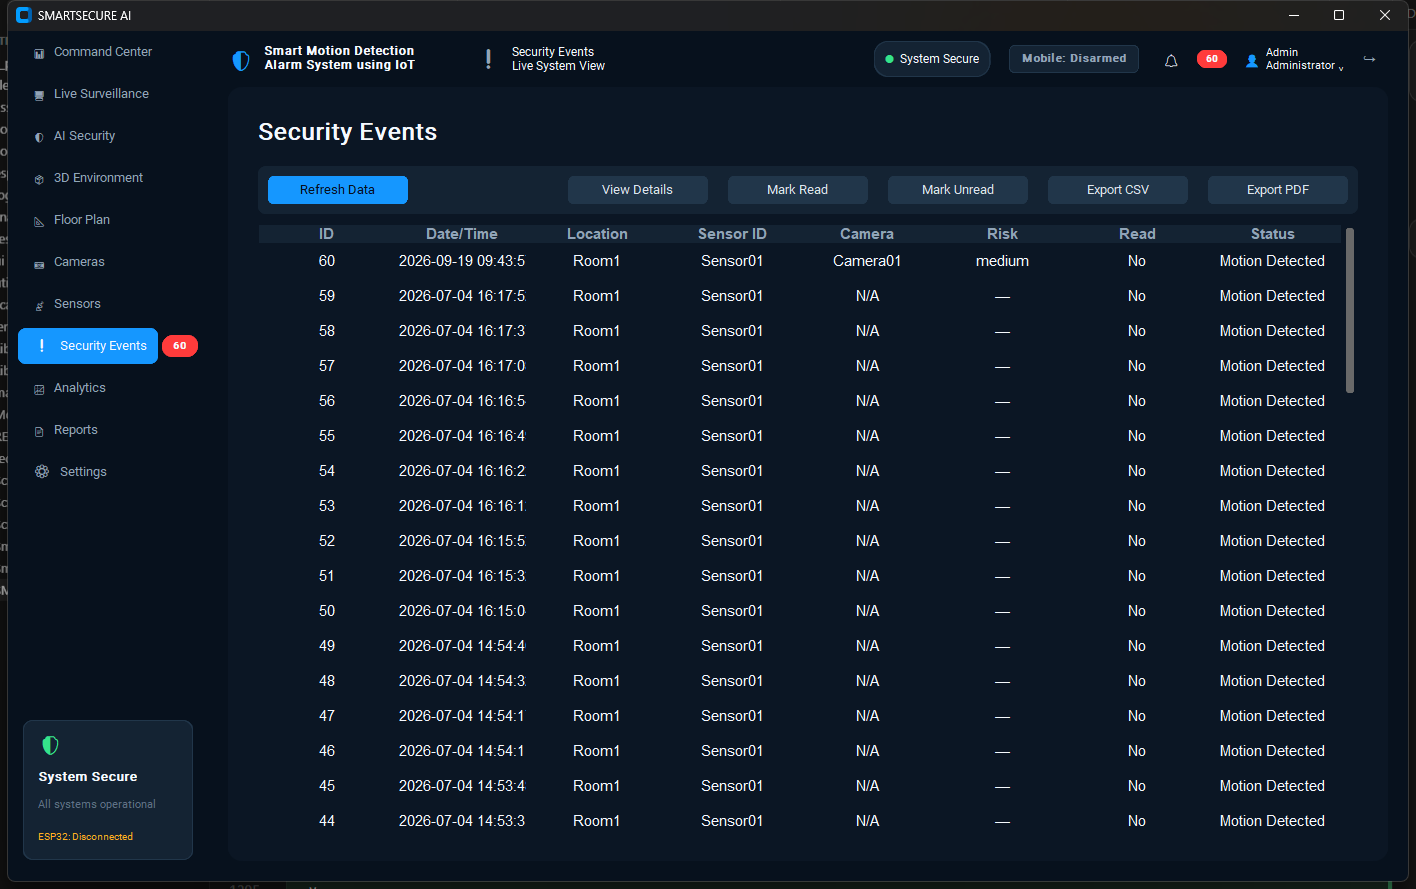
\includegraphics[width=0.88\textwidth]{Screenshot 5.png}
    \caption{Smart Motion Detection Alarm System using IoT -- Security Events}
    \label{fig:screenshot5}
\end{figure}

\begin{figure}[htbp]
    \centering
    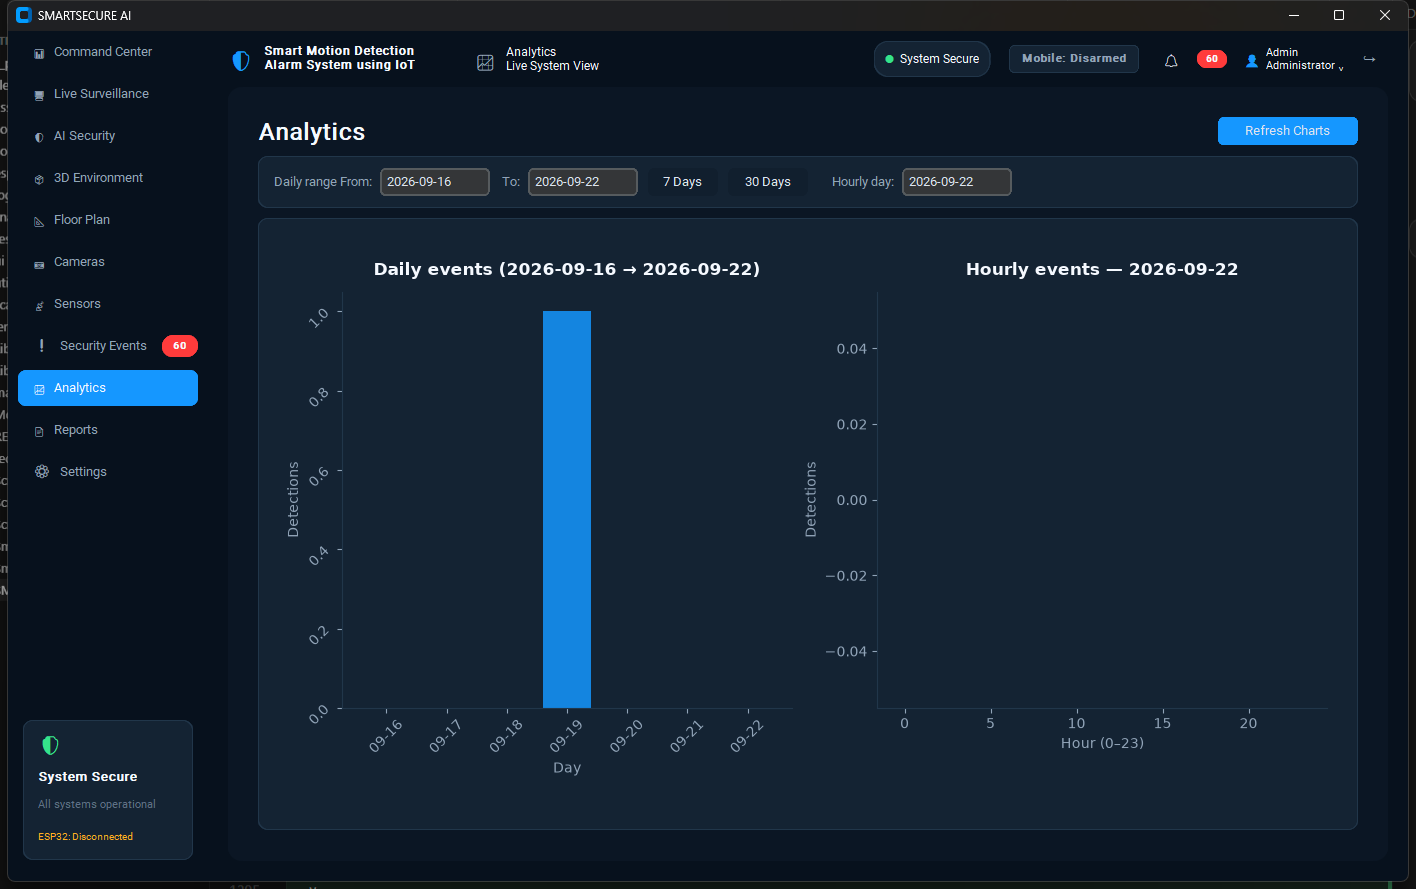
\includegraphics[width=0.88\textwidth]{Screenshot 6.png}
    \caption{Smart Motion Detection Alarm System using IoT -- Analytics}
    \label{fig:screenshot6}
\end{figure}

\newpage

\begin{figure}[htbp]
    \centering
    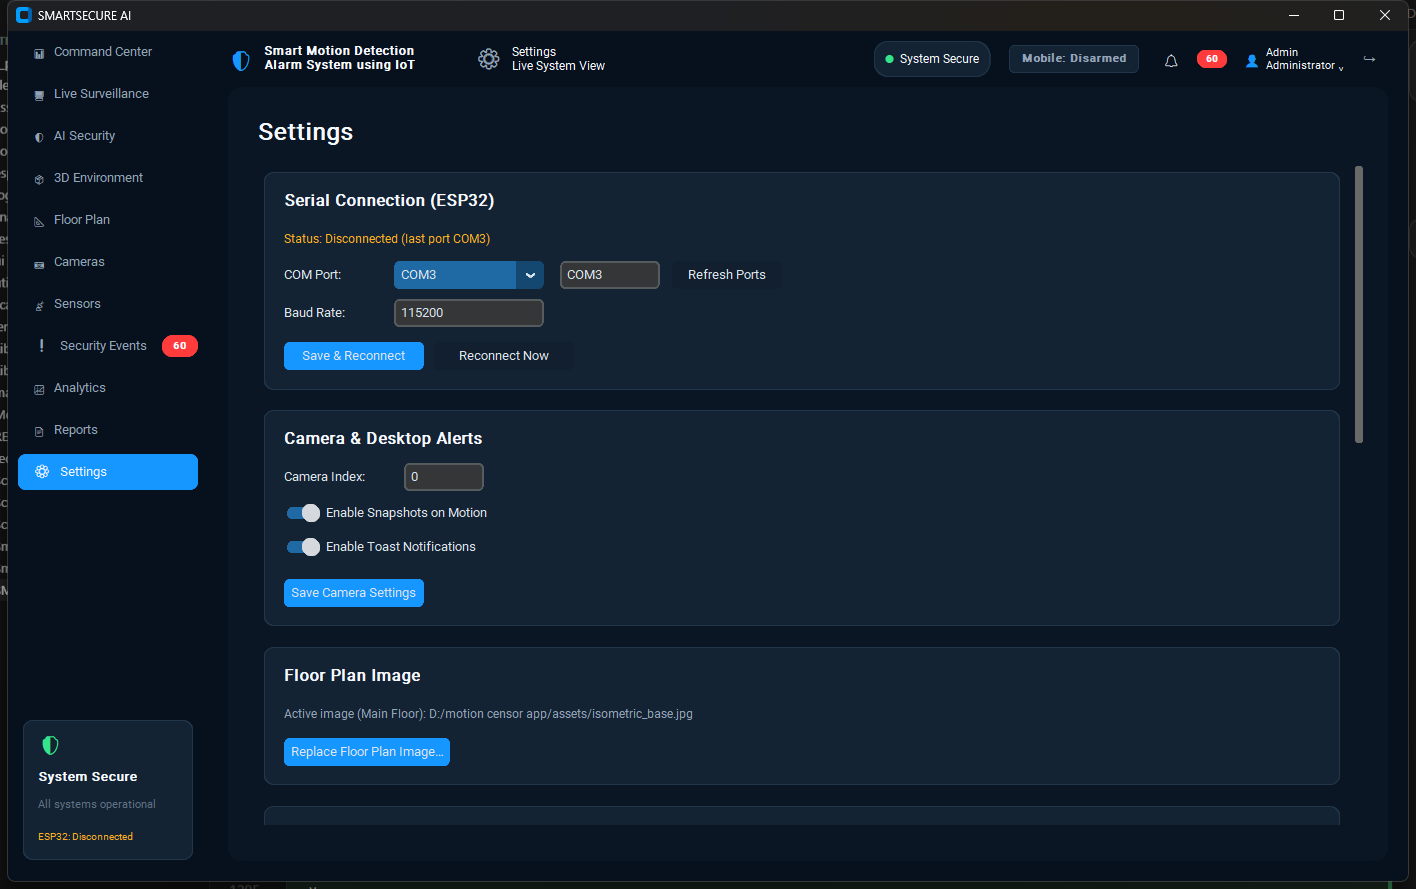
\includegraphics[width=0.88\textwidth]{Screenshot 7.png}
    \caption{Smart Motion Detection Alarm System using IoT -- Settings}
    \label{fig:screenshot7}
\end{figure}

\newpage

\clearpage
\section{Git Logs}

Git logs were kept throughout the development of Smart Motion Detection Alarm System using IoT to track authentication, serial integration, floor-plan features, the motion pipeline, mobile alerts, analytics and reports. They record the main changes made during phases 0--6 of the project.

\vspace{0.5cm}
\begin{figure}[htbp]
    \centering
    \includegraphics[width=1\linewidth]{git1.png}
    \caption{GitHub Repository and Commit History of Smart Motion Detection Alarm System using IoT}
    \label{fig:git-log}
\end{figure}

\end{document}
